%%%%%%%%%%%%%%%%%%%%%%%%%%%%%%%%%%%%%%%%%%%%%%%%%%%%%%%%%%%%%%%%%%%%%%%%%%%%%%%%%%%%%%%%%%%%%%%%%%%%%%%%%%
%%													%%
%% 	BAKALÁŘSKÁ PRÁCE - Začleňování geografických datových sad do OpenStreetMap			%%
%% 				 Martin Jákl								%%
%%													%%
%% pro formátování využita šablona: http://geo3.fsv.cvut.cz/kurzy/mod/resource/view.php?id=775 		%%
%%													%%
%%%%%%%%%%%%%%%%%%%%%%%%%%%%%%%%%%%%%%%%%%%%%%%%%%%%%%%%%%%%%%%%%%%%%%%%%%%%%%%%%%%%%%%%%%%%%%%%%%%%%%%%%% 

\documentclass[%
  12pt,         			% Velikost základního písma je 12 bodů
  a4paper,      			% Formát papíru je A4
  oneside,       			% jednostranný tisk
  pdftex    % překlad bude proveden programem 'pdftex' do PDF
]{report}       			% Dokument třídy 'zpráva'

\linespread{1.3}


\usepackage[utf8x]{inputenc}    % Kódování zdrojových souborů je UTF8x
%\PrerenderUnicode{č,ř,ž,š,ě}    % přidání vyjímky pro znaky s diakritikou
\usepackage[czech]{babel}	% použití češtiny, angličtiny


\usepackage[square,sort,comma,numbers]{natbib}

\usepackage{caption}
\usepackage{subcaption}
\captionsetup{font=small}
\usepackage{enumitem} 
\setlist{leftmargin=*} % bez odsazení

\makeatletter
\setlength{\@fptop}{0pt}
\setlength{\@fpbot}{0pt plus 1fil}
\makeatletter

\usepackage{graphicx} 
\usepackage{color}
\definecolor{purple}{rgb}{0.4,0.0,0.4}

\usepackage{transparent}
\usepackage{wrapfig}
\usepackage{float} 

\usepackage{cmap}           
\usepackage[T1]{fontenc}    

\usepackage{textcomp}
\usepackage[compact]{titlesec}
\usepackage{amsmath}
\addtolength{\jot}{1em} 

\usepackage{chngcntr}
\counterwithout{footnote}{chapter}

\usepackage{acronym}
\usepackage{listings} % nastavení barev pro XML
\lstset{language=XML,
  breaklines=true,
  literate={ý}{{\'y}}1,
  stringstyle=\color{blue},
  identifierstyle=\color{black},
  keywordstyle=\color{purple}\bf,
  morekeywords={osm,way,nd,tag,head,many}}

\usepackage[
    unicode,                
    breaklinks=true,        
    hypertexnames=false,
    colorlinks=true, % true for print version
    citecolor=black,
    filecolor=black,
    linkcolor=black,
    urlcolor=black
]{hyperref}         

\usepackage{url}
\usepackage{fancyhdr}

\usepackage[
  cvutstyle,          
  bachelor           
]{thesiscvut}


\newif\ifweb
\ifx\ifHtml\undefined % Mimo HTML.
    \webfalse
\else % V HTML.
    \webtrue
\fi 

\renewcommand{\figurename}{Obrázek}
\def\figurename{Obrázek}
\pagestyle{empty} % vypne číslování stránek

%%%%%%%%%%%%%%%%%%%%%%%%%%%%%%%%%%%%%%%%%%%%%%%%%%%%%%%%%%%%%%%%%
%%%%%%%%%%% Definice informací o dokumentu  %%%%%%%%%%%%%%%%%%%%%
%%%%%%%%%%%%%%%%%%%%%%%%%%%%%%%%%%%%%%%%%%%%%%%%%%%%%%%%%%%%%%%%%

%% Název práce
\nazev{Začleňování geografických datových sad do~OpenStreetMap}{ Integration of geographic datasets into OpenStreetMap}

%% Jméno a příjmení autora
\autor{Martin}{Jákl}

%% Jméno a příjmení vedoucího práce včetně titulů
\garant{Ing. Martin Landa, Ph.D.}

%% Označení oboru studia
\oborstudia{Geodézie, kartografie a geoinformatika}{}

%% Označení ústavu
\ustav{Katedra geomatiky }{}

%% Rok obhajoby
\rok{2016}

%Mesic obhajoby
\mesic{červen}

%% Místo obhajoby
\misto{Praha}

%% Abstrakt
\abstrakt{
Bakalářská práce se věnuje rešerši problematiky začleňování geografických datových sad kompatibilních s licencí
Open Database License (ODbL) do databáze projektu OpenStreetMap (OSM). Cílem práce je vytvoření metodiky
dávkových importů datových sad publikovaných jako tzv. “opendata” státními institucemi a samosprávou v~ČR do
OSM. Praktická část je zaměřena na problematiku začlenění dat IPR (Institut plánování a rozvoje hl. m. Prahy) a
dalších relevatních zdrojů dat do projektu OSM.
}%
{english/ abstract}

%% Klíčová slova
\klicovaslova
{OpenStreetMap, import, IPR, Python, GDAL}%
{OpenStreetMap, import, IPR, Python, GDAL}

%%%%%%%%%%%%%%%%%%%%%%%%%%%%%%%%%%%%%%%%%%%%%%%%%%%%%%%%%%%%%%%%%%%%%%%%

%%%%%%%%%%%%%%%%%%%%%%%%%%%%%%%%%%%%%%%%%%%%%%%%%%%%%%%%%%%%%%%%%%%%%%%%
%% Nastavení polí ve Vlastnostech dokumentu PDF
%%%%%%%%%%%%%%%%%%%%%%%%%%%%%%%%%%%%%%%%%%%%%%%%%%%%%%%%%%%%%%%%%%%%%%%%
\nastavenipdf
%%%%%%%%%%%%%%%%%%%%%%%%%%%%%%%%%%%%%%%%%%%%%%%%%%%%%%%%%%%%%%%%%%%%%%%

%%% Začátek dokumentu
\begin{document}

\catcode`\-=12  % pro vypnuti aktivniho znaku '-' pouzivaneho napr. v \cline 

% aktivace záhlaví
\zahlavi

% předefinování vzhledu záhlaví
\renewcommand{\chaptermark}[1]{%
	\markboth{\MakeUppercase
	{%
	\thechapter.%
	\ #1}}{}}

% Vysázení přebalu práce
%\vytvorobalku

% Vysázení titulní stránky práce
\vytvortitulku

% Vysázení listu zadani
\stranka{}%
	{\sffamily\Huge\centering\ ZDE VLOŽIT LIST ZADÁNÍ}%
%	{\sffamily\centering Z~důvodu správného číslování stránek}

% Vysázení stránky s abstraktem
\vytvorabstrakt

% Vysázení prohlaseni o samostatnosti
\vytvorprohlaseni

% Vysázení poděkování
\stranka{%nahore
       }{%uprostred
       }{%dole
       \sffamily
	\begin{flushleft}
		\large
		\MakeUppercase{Poděkování}
	\end{flushleft}
	\vspace{1em}
		%\noindent
	\par\hspace{2ex}
	{Chtěl bych poděkovat vedoucímu mé bakalářské práce, Ing. Martinu Landovi,~Ph.D.,
	za odborné rady a~pomoc při zpracování této práce. Dále bych chtěl 
	poděkovat své rodině za projevenou podporu a~trpělivost.}
}

% Vysázení obsahu
\obsah

% Vysázení seznamu obrázků
\seznamobrazku

% Vysázení seznamu tabulek
%\seznamtabulek

% jednotlivé kapitoly
% \setcounter{page}{1}  % nastaví čítač stránek znovu od jedné
\chapter{Úvod}
\label{1-uvod}

K projektu OpenStreetMap (OSM) jsem se dostal již před několika lety.
Zaujala mě možnost sám tvořit a upravovat \uv{mapu}.
Přidávat nové infomace ze svého okolí vlastním sběrem dat
a poté využívat takto vytvořenou mapu.

Postupem času jsem zjistil, co je, a co již není vhodné vkládat do mapy.
Když mi bylo na Fakultě stavební ČVUT v Praze nabídnuto vypracovat
bakalářskou práci na téma, které se dotýká problematiky datových importů OSM,
neváhal jsem. Nedávno totiž Institut plánování a rozvoje hlavního města Prahy
(IPR) uveřejnil všechna svá geografická data.
Tím vznikla možnost začlenit další vhodná data do projektu OSM.

Obsahem této práce je čtenáře nejprve seznámit s projektem
OpenStreetMap. Přiblížit mu vznik a vývoj projektu, užití a jeho licenci.
%%% ML: tato veta nedava smysl, co jste chtel presne rici
Jendá se o cíl, kam se budou importovat zpracovaná data z IPR.
Dále přiblížit problematiku datových importů do OSM a vysvětlit
pojem otevřená data (Open Data).

V praktické části navrhnout aplikaci v programovacím jazyce Python,
která by data poskytovaná IPR umožnila dávkově stáhnout a následně
importovat do pracovní geodatabáze PostGIS a popsat ovládání
vytvořené aplikace.

Následně provést rešerši zveřejněných dat IPR a porovnat je s daty,
která již jsou v OSM. Navrhnout, jaká data by byla vhodná importovat.
V průběhu práce konzultovat tento záměr s~komunitou OSM.
Nakonec vybraná data připravit k~importu z~geodatabáze PostGIS
do OSM.

\chapter{Teorie}
\label{2-Teorie}

\section{OpenStreetMap}
\label{OpenStreetMap}

\subsection{Vznik}
\label{vznik}
OpenStreetMap (OSM) je projekt, jež vznikl s cílem vytvoření a sběru 
volně dostupných geografických dat a následně jejich možné vizualizace
do topografických map. Projekt založil Steve Coast v červenci roku 
2004 v Anglii. Jako inspirace mu posloužil projekt Wikipedia.

Zprvu projekt využívalo jen pár nadšenců, postupem času ale získal
%%% ML: dvakrat "narustat" v jedne vete
projekt popularitu. S nárůstem počtu uživatelů narůstal i objem dat.
%%% ML: nejen kapacitu serveru, ale cele infrastruktury, resit dalsi otazky (bezpecnost a pod)...
Bylo tedy nutné zvyšovat kapacitu serverů. 

V dubnu roku 2006 byla založena nadace OpenStreetMap Foundantion pro financováni 
projektu jako takového (zaměstnanců, běhu serverů atd.). \cite{wikiOSM}


\subsection{Struktura dat}
\label{struktura dat}
OSM data jsou nyní ukládána v databázi PostgreSQL \footnote{viz \url{http://blog.cleverelephant.ca/2009/04/openstreetmap-moves-to-postgresql.html}}
%%% ML: tady to skoro vypada, ze jsou dava ve formatu XML ulozena
%%% primo v DB, cemuz tak ale neni; XML, resp. OSM je vymenny format
a jsou k dispozici ve formátu XML. Jeho výhoda je jasná 
struktura, snadná orientace v kódu pro člověka. Nevýhodou je ovšem větší objem
%%% ML: v jake slova smyslu (prvek ~ soubor) ???
dat, který lze ale snížit kompresí. Každý prvek má vlastní XML soubor. 

%%% ML: tady by se hodil vycet (itemize), chtelo by do vysvetlit, co je cesta a pod...
Třídy prvků v OSM jsou rozděleny na: uzel (node), cesta (way) a
relace (relation).

Příklad XML souboru pro cestu:

{\scriptsize
\begin{lstlisting}
<osm version="0.6" 
generator="CGImap 0.4.0 (32632 thorn-01.openstreetmap.org)" copyright="OpenStreetMap and contributors" attribution="http://www.openstreetmap.org/copyright" license="http://opendatacommons.org/licenses/odbl/1-0/">
   <way id="87249754" visible="true" version="2" changeset="34489106" timestamp="2015-10-07T11:52:41Z" user="Petr Dlouhý" uid="17615">
       <nd ref="1014526199"/>
       <nd ref="1014525941"/>
       <nd ref="1014526337"/>
       <nd ref="1014526022"/>
       <nd ref="1014526277"/>
       <nd ref="1014525984"/>
       <tag k="highway" v="path"/>
       <tag k="source" v="bing:ortofoto"/>
   </way>
</osm>
\end{lstlisting}
}


Uzel je definován jedinečným identifikátorem ({\tt node id=}). Jeho
%%% ML: dodat EPSG kod, vsechny souradnice jsou v jednom SRS...
souřadnice jsou ve WGS~84. Je také ukládána verze ({\tt version= }) a kdy
%%% ML: opet cestina (minimalne 2x "a")... preformulovat
byl do databáze přidán a v jaké změně to bylo provedeno ({\tt changeset=~}).
%%% ML: cely tento odstavec plati i pro dalsi elementy - way/area (?)
Dále k bodu je možné připojit různé atributy s klíčem a hodnotou ({\tt tag~k=~v=~}).

Linie je spojení dvou a více uzlů, dále má také svůj identifikátor ({\tt way~id=~}).
%%% ML: nejde o hlavicku, ale o xml atributy a tagy...
Hlavičku XML souboru má shodnou s bodem. Ale dále obsahuje také seznam id uzlů,
které ji tvoří. Liniím lze taktéž přiřadit atributy.

Linie lze ještě rozdělit na neuzavřené a uzavřené. Uzaveným liniím lze připojit
i atributy určené jen pro plochy. Například les ({\tt landuse=forest}).
%%% ML: veta nize - ?
V případě, když se přidá atribut, který je prot linie, ale chceme
ho použít pro plochy, musí se ještě přidat se atribut {\tt area=yes}.

Speciálním příkladem jsou relace ({\tt relation= }), do kterých lze zahrnout
jeden a více prvků. Lze do nich spojit prvky stejné, nebo odlišné třídy,
nebo i jiné relace. Například dálnice je tvořena několika liniemi (cestami), a ty
jsou zahrnuty do společné relace Dálnice D1. Nebo např. turistická trasa
(od~KČT) je relace sdružující jak linie (cesty, pěšiny) tak i uzly
(rozcestníky, vyhlídky, apod. ).

%%% ML: osm wiki zni familiarne, + reference v tomto pripade je lepsi
%%% hned za slovem, nemusim byt na konco odstravce
U atributů popsaných na osmwiki \cite{OSMfeatures} je vždy uvedeno, k jaké třídě je
vhodné a nevhodné je použít (dle komunity uživatelů OSM). Pokud se stane, že je použit
%%% ML: to ???
na~jinou než povolenou třídu, nemusí to hlásit chybu, ale může být následně
%%% ML: viz kapitola?
problém v některých vykreslovačích. 

\subsection{Změna licence}
\label{změna licence}

%%% ML: Původně vs. původní data...
Původní data OSM a generované grafické dlaždice
byly na distribuovány pod licencí
Creative~Commons~AllributionShare~Alike 2.0 (CC~BY~SA~2.0).

Tato licence umožňovala užití (distribuci ale i editaci) díla pod podmínkou,
že bude uveden zdroj OpenStreetMap.org ve viditelné části
vytvořených mapových dlaždic \cite{OSMlicence}.

  \begin{figure}[hbt]
    \centering
      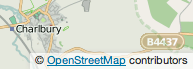
\includegraphics{./pictures/attribution_example.png}
      \caption{Příklad umístění licence}
      \label{fig:attribution_example}
  \end{figure} 

%%% ML: duvod zmeny ?
V roce 2012 byla licence publikovaných dat změněna na Open Data Commons
Open Database Licence (ODbL).
Tato změna licence přinesla problém
s~daty, které byly poskytnuty projektu v předchozí licencí
(CC~BY~SA~2.0). Bylo nutné se dotázat každého z dřívějších
přispěvatelů dat, ať už právnických osob, tak i fyzických osob, jestli
%%% ML: slo o to, zda souhlasi aby jejich prispevky byly poskytovany
%%% pod novou licenci, veta to naznacuje, ale je nepresna
s touto změnou souhlasí a je možné s jejich daty i s novou licencí
nakládat. U přispěvatelů, kteří nedovolili užívání jejich díla
%%% ML: co vymazat - jejich prispevky - preformulovat
pod novou licencí, nebo u těch, co se nevyjádřili, bylo nutné
%%% ML: chybi reference, co znamena zlomek?
z~databáze vymazat. Tato situace nastala pouze ve zlomku případů.
%%% ML: v jake mire? doplnit
Nejvíce tato změna licencí ohrozila data v zemích jako je Polsko a Nový Zéland.

%%% ML: proc tento dualismus?
V současnosti jsou tedy data OSM distibuována pod licencí ODbL a
generované grafické dlaždice pod licencí CC-BY SA 4.0
\cite {OSMlicenceIssue}.

\subsection{Licence ODbL}

%%% ML: preformulovat: Licence ODbl umoznuje...
Ve zkratce s daty pod licencí ODbL uživatel smí:
\begin{itemize}
    \item    kopírovat, distribuovat a užívat data
    \item    vytvářet nová data z původních
    \item    měnit původní data
\end{itemize}

%%% ML: preformulovat
S použitím ale uživatel musí ale uvést zdroj a licenci dat.
Dále uživatel souhlasí, že nová data vytvořená z původních dat budou sířena
také pod~licencí ODbL.
Podrobněji viz přesné znění licence na stránkách OpenDatabase.\footnote{\url{http://opendatacommons.org/licenses/odbl/1.0/}}


\subsection{Zdroje dat}
\label{Zdroje dat}

Jak bylo zmíněno, byla snaha, aby mapová data tvořili jedinci prvotním
sběrem dat, tj. měřením vlastními GNSS (GPS, Glonass) přijímači a
znalostí místních poměrů (uzavřené silnice, stezky atd.).  A takto
vzniklé dílo volně užívat k vlastním potřebám.  Komunita přispěvatelů se
zprvu pomalu, později poměrně rychle rozrostla a dnes čítá 3,7 milionů
registrovaných uživatelů s alespoň jednou vytvořenou změnou v OSM a
2,7 milionů účtů aktivních přispěvatelů.\cite{OSMstats}

Takto vzniklé mapové podklady byly velice vhodné i pro další projekt, dnes již
velice rozšířený a známý jako Geocashing (GC). Projekt GC začal mapové
podklady od OSM užívat a zároveň jeho uživatelé začali sami tvořit a
přispívat do OSM. 

Přispěvatelé dat do OSM musí respektovat licenci projektu OdbL.
Tudíž i jejich zdroj dat musí splňovat tuto licenci. Proto by měli
všechny svoje změny, které v OSM vytvoří, řádně ozdrojovat atributem
s~klíčem 
{\tt source}.
V případě vlastního sběru dat se vyplňuje hodnotou
{\tt source=survey} ,
popřípadně uvést zdroj, odkud čerpali. Pokud tuto povinnost poruší a
použijí zdroj, jež není kompatibilní s licenční politikou OSM, tak ostatní přispěvatelé do OSM tuto změnu, aby předešeli sporům, odstraní. V tomto případě dojde k odstranění celé sady změn, byť by v~ní byl pouze jeden prvek, jenž toto poruší.

%%% ML: nejen soukrome, ale i statni organizace, viz CUZK s RUIANem,
%%% OK mate to v dalsi odstavci
Druhým významným zdrojem dat jsou soukromé subjekty (společnosti).
Většinou jde o podkladové zdroje dat, například ortofoto. Pro obkreslování
silničních síti z~leteckých nebo satelitních snímků. V~jejich případě to
bylo řešeno písemným svolením, nebo smlouvou. Jako významným zdrojem byla
%%% ML: a ted uz neni...? Bing je spolecnost, nevlastni ji MS?
společnost Bing, jež nabídla k~dispozici letecké snímky většiny
obydlené pevniny. 

Třetím zdrojem dat a zároveň postupně dominujícím, co do jeho obsahu, jsou
%%% ML: ze -> produkované
datové sady ze státního sektoru. Tyto datové sady jsou nejvhodnějším zdrojem
%%% ML: proc ? vyargumentovat
dat.

\subsection{Vykreslovače}
\label{Vykreslovače}
Na hlavní stránce OSM (\url{http://www.openstreetmap.org}) je k dispozici mapová aplikace. Ta nabízí pět
„základních“ přednastavených vrstev vykreslených z~dat z OSM. Mapová
%%% ML: na cem je zalozen AJAX, kdyz uz to zminujete. Vysvetlit anebo odstranit.
aplikace OSM využívá knihovnu OpenLayers založenou na konceptu AJAX.
%%% ML: jde o EPSG:3857 - zminit, stejny souradnicovy system pouziva
%%% Google Maps a pod.
Pro snadné vykreslení dat do grafických dlaždic se používá Mercatorovo
zobrazení.

%%% ML: mozna dodat screenshoty do prilohy?
\begin{itemize}

  \item Standardní vrstva - vykresluje všechny prvky přiměřeně.
  \item Cyklomapa - vykresluje cyklostezky, výškopis. 
  \item Dopravní mapa - vykresluje silniční a železniční sítě.
  \item MapQuest Open - podkladová mapa právě pro potřeby 
    Geocaching.
    %%% ML: restaurace na prvni miste?
  \item Humanitární mapa, která vykresluje služby (restaurace, banky, muzea, 
  školy, kostely...)  a potlačuje ostatní prvky. 

\end{itemize}

%%% ML: kompozici? ruznych dat? dovysvetlit
Existují další stránky, jež se zabývají vlastní kompozicí a vykreslením
různých dat. Například mapu turistických a cyklistických tras vykresluje
pro celou Evropu mtbmap.\footnote{mtbmap.cz}

%%% priklad? mozna dodat hezky screenshot?
Zajímavými projekty jsou například ty, které k 2D mapě přidávájí „třetí“ rozměr a
vytvářejí tzv. 2.5D mapu. Většinou jde o 3D zobrazení budov, mostů (dle
atributů), popřípadě i stromů.

\section{Opendata}
\label{opendata}

%%% ML: od kud toto cerpate. Otevrena data (ala public domain) maji
%%% svuj puvod mnohem drive, v devadesatych letech...
Základní myšlenka otevřených dat vznikla v USA z iniciativy vlády Barracka Obamy.
%%% ML: nejen geograficka data
Tedy pokud vzniknou geografická data z veřejných peněz, měla by tedy být
%%% ML: tady neco tvrdite, ale nemate to podlozeno
přístupná veřejně. Mělo to kladný efekt na tamní ekonomiku. Díky tomuto byly
%%% ML: Landsat a SRTM jsou zverejnena jiz delsi dobu... to opravdu
%%% nesouvisi s vladou BO
zprvu k~dispozici satelitní snímky povrchu Země a digitální model terénu
s~rozlišením 30x30 m od NASA (pro pozdější vykreslení vrstevnic).

Tento trend se začal rozšiřovat zprvu do zemí západní Evropy,
%%% ML: druha cast vety nenavazuje na prvni, jake zeme, opet, nejaka
%%% reference?
jmenovitě Velké Británie, Francie či Německa, ale i jiné země mimo Evropu..

%%% ML: Fond se jmenuje Fond Otakara Motejla (opravdu jej zalozil on,
%%% nebyl zalozen na jeho pocet). Jednim z projektu fondu jsou prave
%%% Otevrena data
V ČR se tomuto věnuje fond Otevřená data\footnote{www.otevrenadata.cz}, který založil Otakar
%%% ML: Sociery? co Rekostrukce statu a pod.?
Motejl. Tento fond spolupracuje s nadací Sociery Fund Praha. V rámci
těchto uskupení je vyvíjen tlak na transparentnost veřejné správy a
zveřejňování smluv a dat
státních institucí, jelikož jejich získání a údržba byla placena
z~veřejných zdrojů.



\section{Importy}
\label{Importy}
Výraz import v tomto případě znamená začlenění většího množství datových sad
z~jednoho datového úložiště (databáze serveru) na jiný. Při velkých objemech dat
se využívá výkonu výpočetní techniky z důvodu její bezchybovosti, a také
z~důvodu časové náročnosti. Na člověku poté ale zbývá zvolit postup importu
a naprogramovat skript nebo program, podle něhož technika samotný proces
provede. 

Datové importy z veřejných databází do databáze OSM jsou velmi cenné. 
Otevřené geografické, ale i jiné, databáze státu a jeho veřejných institucí 
financovaných státem jsou komplexní. Komplexní v tom smyslu, že obsahují celistvý
soubor dat, protože je daná instituce vyžaduje ke svém chodu. Jistá nevýhoda tu 
ale může být, a to, že data nemusí být vždy úplně aktuální. Některá data mohou 
být sbírána a zveřejněna i s větším časovým odstupem.

V rámci České Republiky proběhlo již několik hromadných datových importů. Jak 
již bylo řečeno, větší časová náročnost zabere samotná příprava na import. A to
v~případě, importu do OSM. Nejen napsání skriptu, ale i nutná diskuze tohoto záměru
na~diskuzní konferenci Talk-cz. 

\subsection{Talk-cz}
\label{Talk-cz}
Tato diskuze probíhá přes posílání emailových zpráv do společné konference. 
Uživatelům chodí emaily z probíhající diskuze a pokud na nějaký chtějí reagovat,
tak pošlou email na adresu serveru, na kterém diskuze běží, a musí do Předmětu 
napsat Re: a předmět zprávy, na kterou reagují. Server tyto zprávy pomocí 
předmětu a času řadí. Diskuze je poté k dispozici na webových stránkách.\footnote{http://lists.openstreetmap.org/listinfo/talk-cz}

\section{IPR Praha}
\label{IPR Praha}
IPR Praha je zkratka názvu Institut plánování a rozvoje a hlavního města Prahy. 
Tento institut se věnuje urbanismu, architektury a rozvoje města Prahy. Hlavním
úkolem IPR je tvorba územního plánu Prahy a významným úkolem IPR je zajišťovat
zpracování geografických informací. Spravuje data a mapy města Prahy. Od roku 
2002 poskytuje na svých stránkách zdarma webové aplikace bez limitu využití. 
Po~rozvoji Pražského geoportálu došlo k jejich většímu využívání.  Na základě 
platných Pravidel pro poskytování dat a  výstupů z datových souborů a datového 
skladu Geografického byla od dne 1.~4.~2015 zveřejněny datové soubory a další 
webové služby. Tato data byla uveřejněna pod licencí CC-BY SA 4.0 \cite{IPR}
\subsection{licence CC BY-SA 4.0}
\label{licence CC BY-SA 4.0}
Licence CC BY-SA 4.0 je zde uvedena ve zjednodušeném znění.

"Uživatel s smí
\begin{itemize}
    \item   Sdílet - rozmnožovat a distribuovat materiál prostřednictvím jakéhokoli média v jakémkoli formátu
    \item   Upravovat - remixovat, změnit a vyjít z původního díla
\end{itemize}
pro jakýkoliv účel, a to i komerční.

Poskytovatel licence nemůže odvolat tato oprávnění do té doby, dokud dodržujete licenční podmínky.

Uveďte původ — Je Vaší povinností uvést autorství, poskytnout s dílem odkaz na licenci a vyznačit Vámi provedené změny. Toho můžete docílit jakýmkoli rozumným způsobem, nicméně nikdy ne způsobem naznačujícím, že by poskytovatel licence schvaloval nebo podporoval Vás nebo Váš způsob užití díla.

Zachovejte licenci — Pokud budete toto dílo upravovat, pozměňovat nebo na něj navazovat, musíte svoje odvozená díla vystavovat pod stejnou licencí jako původní dílo."

Podrobněji viz přesné znění na stránkách CraetiveCommmons.
\footnote{https://creativecommons.org/licenses/by-sa/4.0/legalcode/}


\section{PostgreSQL}
\label{PostgreSQL}
PostgreSQL je Opensource databázový systém, který je vyvýjen déle než patnáct
let. Za dlouhou dobu vývoje se stal robustní a také hojně využívaný.
Postupem času získal svou spolehlivostní silnou reputaci.
Lze s ním pracovat ve všech známých operačních systémech. 
...
\cite{PostgreSQL}

\subsection{PostGIS}
\label{PostGIS}
PostGIS je objektově-relační nadstavba databázové struktury PostgreSQL.
Rozšiřuje ji o funkce, které umožňují geometrické operace s objekty v ní uložené.
Třídy prvků mohou být buď bod (point), linie (line) nebo polygon (polygon).
Dále je možné více prvků jedné třídy sdružit do multi-relace, 
to jest  multiPoint, multiLine, multiPolygon.
Geometrie prvku určuje jeho polohu v určité souřadnicové soustave, neboli 
kartografickém souřadnice. Dále určuje i kartografickou soustavu, ve které je 
jeho geometrie určena. Je tedy dále možné při známých transformacích mezi
soustavami provádět transformace souřadnic. Základní operace jako délka, obvod,
plocha, ale jsou zde i sofistikovanější funkce, které lze s objekty nebo i mezi 
objekty provádět.

Sotware PostGIS je šířen pod GNU General Public License (GPLv2) licencí.


\section{Python}
\label{Python}
Programovací jazyk Python vznikl v roce 1991. Navrhlo ho Guido van Rossum. 
Je vyvíjen jako open source projekt. Inspiroval se hlavně programovacím jazykem
ABS, který byl přímo vytvořen pro~výuku začatečníků v programování. Python je 
proto jeden z nejvýhodnějších programovacích jazyků pro začínající programátory,
ale i přesto ho lze použít pro~praktické programování. 

Jedná se tedy o jednoduchý programovací jazyk podporující různá programovací 
paradigmata, hlavně objektové, imperiativní, procedurální a omezené míře i 
fun- kcionální. Je multiplatformní, lze jej tedy použít na různých operačních 
systémech. Klade velký důraz na syntaxi psaného kódu, využívá hlavně prázdné 
znaky v~psaném kódu.  

Programy nebo skripty lze psát v textovém editoru, ale je vhodné použít 
standartu PEP~8, který kontroluje prázdné znaky a správnou strukturu skriptu. 

V současné době je vydána stabilní verze 3.5.7, která vůči předchozí verzi 2.x
mění některá, již "zažitá" syntaxe. Například nejviditelnější je změna funkce 
{\tt print } pro verzi 2.x stačilo  {\tt print 'Ahoj'}  a pro verzi 3.x je již
nutné string vložit do závorek  {\tt print('Ahoj')}  . Tyto dvě dnes používané
verze 2.x a 3.x jsou navzájem nekompatibilní.
\cite{python} 
\cite{wikiPython} 
  
  
\subsection{knihovna argparse}
\label{argparse} 
Knihovna argparse, jejíž autor je Tshepang Lekhonkhobe, je knihovna 
do~programovacícho jazyku Pyhon. Řeší konzolový vstup do aplikace a zpracovává 
ho pro další použití v programu.\cite{argparse}


\subsection{knihovna xmltodict}
\label{xmltodict} 
Tato knihovna umí číst soubory ve formátu XML a zpracovává je do snažší formy 
dat, která je jednodušší manipulaci pro samotný program. Data z XML zpracuje
do formy datové řady (array), kde každý člen této řady může být opět řada dat.\cite{xmltodict}

příklad parsování dat ve XML formátu

{\scriptsize
\begin{lstlisting}
<head>
  <many>ele1</many>
  <many>ele2</many>
</head>
\end{lstlisting}
}

Po otevření a parsování se v Python(u) provede příkazem.

{\scriptsize
\lstset{language=Python}
\begin{lstlisting}
with open('example.xml') as fd: 
  doc = xmltodict.parse(fd.read()) 
\end{lstlisting}
}

Objekt {\tt doc} má poté podobu.

{\scriptsize
\lstset{language=Python}
\begin{lstlisting}
OrderedDict([(u'head', OrderedDict([(u'many', [u'ele1', u'ele2'])]))]) }
\end{lstlisting}
}

V této datové řadě lze již snadno procházet. 

{\scriptsize
\lstset{language=Python}
\begin{lstlisting}
doc['head']['many'][0]
ele1
\end{lstlisting}
}


\subsection{knihovna GDAL/OGR}
\label{GDAL/OGR}
Jedná se o knihovnu pro práci s geografickými daty a umožňuje jejich čtení a zápis.
Je psána v programovacím jazyce C++. Je považován za jeden z hlavních 
open~source projektů a je hojně používán ve sféře GIS. Pracuje s vektorovými a 
rastrovými datovými formáty. Podporuje velkou škálu souborových formátů, a to 
pro vektorová data, ale i pro rastrová. Obsahuje databázi definic kartografických
projekcí používaných na celém světě a databázi jejich známých transformací. 
Umožňuje tedy komplexní operace s geografickými daty. \cite{GDAL}


\section{QGIS}
\label{QGIS}
QGIS je program vytvořen za účelem prohlížení a editace geografických dat.
Jedná se o Opensource software. Je tedy možné, aby na jeho vývoji spolupracoval
kdokoli. Je možné si vytvářit novou funkci, nebo přímo zásuvný modul do programu.
Je možné je psát v jazyce C++ nebo Python.
Tyto moduly si uživatelé mohou poté stáhnout a přidat do QGISu a využívat.
QGIS také umožňuje využívat konzolově jazyk Python. Je možné si tak vytvářet
vlastní jednoduché skripty v jazyce Python a spouštět je v QGISu.

Od svého vzniku bylo vydáno již spoustu verzí programu.
Dříve byly verze pojmenovávány podle planet, později podle jejich měsíců a nyní se dávají
jména německých měst. V současnosti (duben 2016) je k dispozici verze 2.14 Essen

\chapter{Použité technologie}
\label{3-technologie}

\section{PostgreSQL}
\label{PostgreSQL}

PostgreSQL je open source objektově-relační databázový systém. Za dlouhou dobu vývoje se stal robustním a hojně využívaným řešením hlavně díky své spolehlivosti. Lze s ním pracovat ve všech známých operačních systémech. 
\cite{PostgreSQL}

\subsection{PostGIS}
\label{PostGIS}
PostGIS je nadstavba databázového systému PostgreSQL.
Rozšiřuje jej o funkce a~datové typy, které umožňují uložení, manipulaci a správu geografických objektů. Mezi podporované geometrické typy patří bod (point), linie (linestring),
nebo polygon (polygon). Dále je možno prvky sdružit 
do tzv. multiprvků (multiPoint, multiLineString nebo multiPolygon). Geometrie prvku určuje
jeho polohu v daném souřadnicovém systému. Data je tedy možno transformovat do jiných PostGISem podporovaných souřadnicových systémů. Systém kromě základních operací jako výpočet délky, obvodu, plochy, podporuje i sofistikovanější funkce jako je např. výpočet obalové zóny a další.

Sotware PostGIS je šířen pod GNU General Public License (GPLv2).

\section{Python}
\label{Python}
Programovací jazyk Python vznikl v roce 1991. Navrhl ho Guido van
Rossum. Je vyvíjen jako open source projekt. Inspiroval se hlavně
programovacím jazykem ABS, který byl přímo vytvořen pro~výuku 
začátečníků v programování. Python je proto jeden z nejvýhodnějších
programovacích jazyků pro začínající programátory, ale i přesto ho lze
použít pro~praktické programování.

Jedná se o jednoduchý programovací jazyk podporující různá
programovací paradigmata, hlavně objektové, imperativní, procedurální
a v~omezené míře i funkcionální. Je multiplatformní, lze jej tedy
použít na~různých operačních systémech. Klade velký důraz na~syntaxi 
psaného kódu, využívá hlavně prázdné znaky v~psaném kódu.

Programy nebo skripty lze psát libovolném textovém editoru. Vhodné je
použít standardu PEP~8, který definuje správnou strukturu odsazení kódu.

V současné době je vydána stabilní verze 3.5.7, která oproti předchozí
verzi 2.x mění některé již \uv{zažité} vlastnosti jazyka. Například 
nejviditelnější je změna funkce {\tt print()}. Ve verzi 2.x stačilo napsat
 {\tt print 'Ahoj'}. Ve verzi 3.x je již nutné řetězec vložit
do~závorek  {\tt print('Ahoj')}. Tyto dvě dnes používané verze 2.x
a 3.x jsou navzájem nekompatibilní.
\cite{python} 
\cite{wikiPython} 
  
\subsection{Knihovna argparse}
\label{argparse} 
Knihovna argparse je knihovna 
programovací jazyka Python, která řeší konzolový vstup do aplikace a 
zpracovává ho pro~další použití v programu.\cite{argparse}

\subsection{Knihovna xmltodict}
\label{xmltodict} 
Tato Python knihovna umí číst soubory ve formátu XML a zpracovat jejich obsah do datové struktury, která je jednodušší pro manipulaci v samotném
programu. Data z~XML zpracuje do~slovníku (dictionary), kde klíčové slovo (key) reprezentuje hodnota(value) ve slovníku.
Hodnotami mohou být dále i řady dalších klíčových slov (key).\cite{xmltodict}

Příklad zpracování dat ve formátu XML.

{\scriptsize
\begin{lstlisting}
<head>
  <many>ele1</many>
  <many>ele2</many>
</head>
\end{lstlisting}
}

Zpracování dat provedeme v Pythonu příkazem:

{\scriptsize
\lstset{language=Python}
\begin{lstlisting}
with open('example.xml') as fd: 
  doc = xmltodict.parse(fd.read()) 
\end{lstlisting}
}

Objekt {\tt doc} vypadá následově:

{\scriptsize
\lstset{language=Python}
\begin{lstlisting}
OrderedDict([(u'head', OrderedDict([(u'many', [u'ele1', u'ele2'])]))]) }
\end{lstlisting}
}

Data v této struktuře lze již jednoduše procházet.

{\scriptsize
\lstset{language=Python}
\begin{lstlisting}
doc['head']['many'][0]
ele1
\end{lstlisting}
}

\subsection{Knihovna GDAL}
\label{GDAL}
Jedná se o knihovnu pro práci s geografickými daty umožňující jejich
čtení a~zápis. Je napsána v programovacím jazyce C++. Je považována
za~jeden z hlavních open~source projektů hojně využívaných ve~sféře
GIS. Podporuje velkou škálu rastrových a vektorových formátů.
Díky knihovně PROJ.4 podporuje celou škálu souřadnicových systémů a umožňuje transformaci dat mezi nimi. \cite{GDAL}

\section{QGIS}
\label{QGIS}
QGIS je program vytvořený za~účelem prohlížení a editace geografických
dat. Jedná se o open source software. Je tedy možné, aby na~jeho vývoji
spolupracoval kdokoli. Vlastní uživatelské nástroje se píší ve formě tzv. zásuvných modulů, které je možné implementovat v jazyce C++ nebo Python.
Tyto moduly si ostatní uživatelé mohou poté stáhnout a začlenit do své instalace QGISu. QGIS také umožňuje využívat jazyk Python v rámci vestavěné konzole. Lze tak vytvářet vlastní jednoduché skripty v jazyku Python a spouštět
je přímo v~QGISu.

Od svého vzniku byla vydána již spousta verzí tohoto programu. Dříve byly
verze pojmenovávány podle měsíců planet Jupitera a Saturnu, později se začaly používat jména měst. V současnosti (duben 2016) je
k~dispozici verze 2.14 Essen.

\chapter{Praktická část}
\label{4-Praktická část}

\section{Geodatabáze PostGIS}
\label{Server PostGIS} 
V rámci této bakalářské práce byla zřízena geodatabáze PostGIS na školním
serveru {\em geo102}. Data z OSM jsou do školní databáze nahrávána pomocí programu {\tt osm2pgsql}.\footnote{dostupné z \url{http://wiki.openstreetmap.org/wiki/Osm2pgsql}}
%%% ML: to neni pravda, shellovy skript (viz git) pracuje primo s daty CR
%Ten nejprve stáhne aktuální data pro celou Evropu a následně je ořeže
%jen na území ČR.
%%% ML: neskodilo by zminit, ze tyto aktualnize zajistuje shellovy skript, ktyery je soucasti prilohy na cd
Obsah databáze je každý den pravidelně aktualizován podle aktuálního stavu OSM.

%%% ML: my jsme to zakladni schema ale upravovali (height)
Tabulky v databázi byly vytvořeny podle základního schématu. Pro~každou třídu prvků (uzel, cesta
a relace) je vytvořena samostatná tabulka. Pro~uzly je vytvořena
tabulka {\tt czech\_point}, pro~cesty tabulka {\tt czech\_line} a pro~plošné prvky (uzavřené cesty s atributy
pro~plochy) tabulka {\tt czech\_polygon}. Relace jsou
%%% ML: plochami a ne plochamy! (to uz me prekvapilo, rikal jste, ze text projde jazykovou korekci)
řešeny tak, že pokud jsou tvořeny plochami, vytvoří z~nich program
{\tt osm2pgsql} multipolygon a ten vloží do~tabulky {\tt czech\_polygon}. Stejně jsou
řešeny i relace tvořené cestami (tabulka~{\tt czech\_line}), respektive body
({\tt czech\_point}). Ještě je dle schematu vytvořena tabulka
{\tt czech\_roads}, která obsahuje všechny silnice v~ČR.

Každý prvek má přiřazen, v~rámci tabulky, jedinečné číslo {\tt gid}.
Dále je vytvořena pro každý prvek geometrie a pro~každý
atribut (dle schématu) stejnojmenný sloupec s~hodnotou. Například
bod s~atributem {\tt landuse=forest} má ve~sloupci {\tt landuse}
hodnotu {\tt forest}.

Takto vytvořená databáze bude použita pro~analýzu dat IPR a~jejich přípravu pro importu do~OSM.

\section{Data IPR}
\label{IPR data}
%%% ML: zde by se hodila reference na kap., kde o tom pisete
IPR na svém webu od~jara roku 2015 zveřejňuje svá data v režimu otevřených dat. Vektorová data zveřejňuje ve formátech GeoJSON, DXF, GML a ESRI Shapefile. Dále je na~výběr mezi dvěma
%%% ML: jsou to srs ane kartograficka zobrazeni (jste studenten geodezie!)
souřadnicovými systémy S-JTSK (EPSG:5514) nebo WGS 84 (EPSG:4326).

Celkem IPR zveřejňuje (toho času) 96 datových setů, které jsou rozděleny
do~kategorií.\footnote{viz webové stránky IPR, \url{www.geoportalpraha.cz/cs/opendata}}

Pokud není řečeno jinak, jedná se o data ve vektorové formě.
Těmito kategoriemi jsou:

\begin{itemize}
    \item   3D model - Obsahuje 3D modely budov a mostů v Praze a
            digitální model povrchu (DMP), dále rastrově digitální
            model povrhu a terénu, absolutní a relativní výšky budov.

            Z těchto dat by se pro OSM dala využít poloha budov
            ze~souboru Budovy 3D. Budovy byly do OSM již importovány
            %%% ML: mate nekde zkratku vysvetlenu
            ze~zdroje RÚIAN, není třeba je tedy importovat znovu.

    \item   Digitální technická mapa Prahy - zde jsou k dispozici
            ve~vektorové podobě všechny inženýrské sítě v~Praze,
            technické budovy a parcelní hranice.

            Do OSM se, možná zatím, nepřidávají inženýrské sítě.
            V~současnosti lze ale do OSM přidávat zdroje veřejného osvětlení.
            %%% ML: nasledujici veta je uplne zbytecna, jsou takovato data v IPR?
            %Takže pokud by nějaký soubor dat obsahoval
            %značky veřejného osvětlení, mohla by se tato
            %data importovat do OSM.
            Hranice města Prahy a jeho městských
            částí již v~OSM jsou dostupná. Datovou sada Technické budovy by bylo
            možné použít jako zdroj pro budoucí aktualizaci OSM.
            %%% ML: no prubehy hranic parcel obsahuje RUIAN, neni treba nic obkreslovat, to se mozna delo drive, dnes jiz rozhodne ne...
            Průběhy hranic parcel lze již nyní bezproblémově
            obkreslovat z rastrových podkladů, které veřejně
            poskytuje ČÚZK. 

    \item   Doprava - obsahuje cyklistické trasy a značky, pěší trasy,
            parkovací zóny, automaty, P+R parkoviště a mapy zón PID.
            Cyklistické trasy v Praze lze do OSM importovat, jsou ale
            %%% ML: uzivateli (a ne uzivately)! vedouci prace neni jazykovy korektor ;-)
            již velmi dobře zmapované samotnými uživateli. Datová sada
            obsahuje bodové značky, z~těch by se některé mohly
            importovat. V~případě datové sady 
            Cyklistická doprava~-~značky, byla data prohledána. Dle IPR
            uváděné hodnoty {\tt 103} ve sloupci {\tt DRUH}
            pro~Bikesharing, bohužel žádné takové hodnoty
            neobsahovaly. Import dat z této datové sady nebyl proto
            dál brán v potaz. Bylo by možné do OSM přidat parkovací
            zóny (jako nový atribut u~stávajících komunikací).
            Vhodná data jsou parkovací automaty a také P+R parkoviště.

    \item   Geologie - obsahuje vektorové mapy radonového nebezpečí.
            Tato data se do~OSM nepřidávají.

    \item   Hluk - obsahuje hlukové mapy, a to ve~dne a v~noci. Oboje
            v~rastrové formě. Tato data se do OSM nepřidávají. Dále
            obsahuje i protihlukové bariéry, které by bylo možné
            do~OSM přidat.

    \item   Kvalita životního prostředí - obsahuje datovou sadu
            Oblasti svozu komunálního odpadu. Tato data není vhodné
            do~OSM začlenit. Dále ale obsahuje datovou sadu
            Odpadní Zařízení pro občany, která obsahuje informace
            o~všech sběrnách odpadu v~Praze. Tato datová sada se jeví
            jako další vhodná pro~import.

    \item   Mapové podklady - obsahuje klady mapových listů různých
            měřítek (1:500 až 1:10~000). Klady mapových listů nejsou
            vhodná data pro~OSM. Dále kategorie obsahuje i datové sady
            vrstevnic, a to po~5~m, 2~m a 1~m. Vrstevnice přímo OSM
            neobsahuje, avšak byly by velkým zpřesněním stávajícího
            zdroje vrstevnic. Nebo jako zdroj pro~projekty, které
            kombinují OSM s~jinými daty.\footnote{Projekt mtbmap.cz nebo \url{http://mapa.prahounakole.cz/}}

    \item   Občanská vybavenost obsahuje pouze datovou sadu Veřejné
            toalety. Jistě jsou již toalety v Praze částečně
            zmapovány, ale i tak by bylo vhodné je doplnit. Jsou tedy
            vybrána jako další vhodná data pro~import.

    \item   Ochrana přírody a krajiny, obsahuje data o ochranných
            pásmech památných stromů. Bohužel ne samotné stromy.
            Vhodná data pro import jsou z~datové sady Přírodní parky a
            Významný krajinný prvek - registrovaný. Z těchto datových
            sad by se mohly doplnit, nebo aktualizovat data v OSM.

    \item   Ortofoto obsahují letecké snímky (rastr) Prahy 
            s~rozlišením až 5~cm na~pixel jak ve~viditelném spektru
            světla, tak i v~infračerveném.

            Ortofoto je vhodné pouze jako podkladový zdroj,
            například pro mapovací aplikaci JOSM.

    \item   Ovzduší obsahuje vektorové mapy znečištění ovzduší a také
            zdroje znečištění. Tato data se v OSM nemapují, jediné co
            by se mohlo přidat do OSM jsou bodové zdroje, a to
            například značkou pro~komín. Dále jsou v~této kategorii i
            bonity, a to z~různých hledisek (ovzduší, půdy,
            osvit, atd.). Tato data nejsou vhodná pro import do~OSM.

    \item   Platný územní plán. V této kategorii jsou datové sady
            Veřejně prospěšných staveb (plošné, liniové a bodové).
            Datová sada VPS obsahuje také informace o~P+R u~stanic
            metra. Tyto informace pocházejí z~územního plánu, a tedy nemusí být
            realizovány. Po prozkoumání a porovnání s~datovou sadou
            Záchytná parkoviště P+R, lze konstatovat, že jsou všechny záznamy obsaženy již v této datové sadě.

    \item   Socioekonomická data obsahuje pouze vektorovou mapu ceny
            pozemků. Data o ceně pozemků se do~OSM nepřidávají. 

    \item   Technická infrastruktura - vodní hospodářství, obsahuje
            záplavová území Q20, Q50 a Q100 a území zaplavené
            povodněmi v roce 2013. Informace o záplavových územích se do~OSM
            nepřidávají. Dále jsou v této kategorii datové sady
            Protipovodňové ochrany, které obsahují údaje o všech dočasných
            protipovodňových zdech. Jelikož se jedná o~dočasné překážky, a to~ještě jen v~době povodně, nemá smysl je do OSM přidávat.

    \item   Urbanismus - Z~této kategorie by se mohly pro OSM využít
            informace z~datové sady
            Stavební uzávěry - dopravní. Bylo by ale nutné udržovat
            aktuálnost infomací o plánovaných dopravních uzavírkách.
            Dále by bylo ještě možné přidat do OSM počet pater budov
            z~datové sady Podlaživost.
\end{itemize}


\subsection{Licenční problém}
\label{Licenční problém}
Jak již bylo řečeno výše, IPR svá data zveřejnil a stále zveřejňuje
(v době tvorby této práce) pod~licencí CC~BY-SA~4.0, viz kapitola \ref{licence CC BY-SA 4.0}.

%%% ML: tak co, vete chybi druha polovina (duvod: tyto dve licence nejsou kompatibbilni)
Jelikož jsou ale data OSM distribuována pod licencí ODbL (v1.0), která
neumožňuje začletnit data z licencí CC BY-SA. 

Na některá data (informace), jako například místní názvy, ulice atd.
se nemohou vztahovat autorská práva. Neboť nevyžadují žádnou 
kreativitu pro jejich \uv{vytvoření}. Ovšem na soubor (databázi) těchto dat
vytvořený podle daných kritérií již může být právní
ochrana uplatněna. A právě proto vznikla licence ODbL, která se
zaměřuje na ochranu databáze jako celku.

U dat chráněných autorským právem a danou licencí se vyžaduje jejich
vzdání. V~některých zemích, kde se nelze úplně vzdát autorských
práv, se vyžaduje omezení autorských práv na~nejnižší možnou
míru. Autor souhlasí, že nebude vymáhat svoje autorská práva, po dobu,
kdy jsou data uložena v databázi. \cite{ODbl}

IPR byl kontaktován, zdali by mohla být jeho data použita do OSM.
Dle vyjádření vyplynulo, že IPR by neměl problém s použitím svých dat,
jelikož jsou zveřejněna pod myšlenkou Opendata. Byla navrhnuta
možnost udělit od~IPR pro~OSM licenční výjimku.

Vznikla by tu však situace, kdy by byla data IPR k dispozici 
pod~licencí CC BY-SA a v~OSM (sice modifikovaná) pod~licencí
ODbL. Tohoto dualismu by mohl využít někdo, komu by licence CC BY-SA
neumožňovala jeho záměr. Mohl by si totiž data obstarat z databáze OSM,
sice modifikovaná, ale již pod novou licencí (ODbL), která by mu jeho
záměr umožnila.

Hlavní rozdíl je totiž v tom, že pod licencí CC~BY-SA sice může data
různě měnit a upravovat, ale poté když je zveřejňuje, musí zachovat
licenci CC~BY-SA. Nemusí ale uvolnit (zveřejnit) data, která k nim 
přidal. V~případě licence ODbl se tato situace diametrálně liší.
Uživatel opět smí data upravovat nebo k~nim přidávat jiná data, ale
poté může svoje dílo distribuovat pod~jinou licencí, za~podmínek, že
uvolní veškerá data, která k tomu použil.

Vhodnější by tedy bylo, změnit licenci dat zveřejňovaných IPR
na~ODbL.

%%% ML: nepredbihal bych, je to spise spekulace
%Dle vyjádření se tato situace bude ze strany IPR řešit tak,
%že se změní licence u distribuovaných dat na ODbL. Tato změna
%licencování se očekává v~několika měsících.


\section{IprDownloader}
\label{IprDownloader}
Jak již bylo řečeno, tak IPR distribuje geografická data ve formě datových souborů stažitelných z webových stránek organizace.
Kromě samotných datových souborů je k~dispozici kanál ve formátu ATOM ({\tt http://opendata.iprpraha.cz/feed.xml}).
Pomocí něho se lze také dostat ke všem distribuovaným datům. Jelikož
by bylo zdlouhavé stahovat všechny tyto soubory ručně, byl
v rámci práce vytvořen program, který umožňuje stahování a také import dat primárně do geodatabáze PostGIS. Skript byl
%%% ML: zde by se hodil odkaz do teoreticke casti
napsán v~programovacím jazyce Python a využívá knihovny GDAL.

Zdrojový kód programu je rozdělen do tří souborů: 
{\tt IprDownloader.py}, \newline {\tt IprBase.py} a {\tt IprPg.py}.


\subsection{IprDownloader}
Skript {\tt IprDowloader.py} parsuje vstupní údaje a
zpracovává je k~dalšímu použití v programu, viz \ref{argparse}. Základními parametry programy jsou
{\tt ---alike, ---crs, ---format, ---outdir, ---d}.
Dalšími vstupními parametry mohou údaje o databázi, kam se mají data
importovat. Jde o 
{\tt ---dbname, ---dbschema, ---dbhost, ---dbport, ---dbuser, ---dbpassword}.

%%% ML: kartografickych souradnic ? (student geodezie by mel znat
%%% rozdil mezi kartografickym zobrazenim a souradnicovym systeme)
%%% Cely odstavec mi neda smysl, zatim jsem jej zakomentoval
%% Skript hlídá vstupní formát kartografických souřadnic, a pokud se
%% neshodují s~možnými, oznámí chybu o špatném vstupu. Pokud uživatel
%% vloží kartografické zobrazení ve formě EPGS kódu, program jej převede
%% na~jeho název.


\subsection{IprBase}
Skript {\tt IprBase.py} definuje třídu {\tt IprDownloader} se všemi
potřebnými funkcemi. Většina funkcí slouží pro otevírání, čtení a
parsování XML souborů, viz kapitola \ref{xmltodict}. Obsahuje funkci
pro~hledání, která prochází všechny záznamy v ATOM souboru a porovnává, zda název
definovaný parametrem {\tt alike} je obsažen v názvu souboru dat. Poté najde dle nastavení ({\tt
  crc, format}) daný soubor a stáhne jej do~definovaného adresáře.


\subsection{IprPg}
Skript {\tt IprPg.py } definuje třídu {\tt IprDownloaderPg}, která
dědí všechny metody rodičovské třídy {\tt IprDownloader } a definuje další
funkce potřebné pro~správný import stažených dat do databáze
PostgreSQL. Přesněji stažený soubor zkontroluje, jestli není 
komprimován v~archivu {\tt *.zip}, pokud ano, tak vytvoří nový adresář,
který má stejný název jako archiv. Do nově vytvořeného adresáře poté 
extrahuje všechna data z archivu.


\section{Ovládání}
Při spuštění vypíše program všechna nalezená data,
která IPR dává k~dispozici. Pro hledání a označení, která data se mají
stáhnout, slouží parametr {\tt ---alike}. Pokud hledaný řetězec obsahuje mezeru,
tak je nutné jej umístit do uvozovek. Program rozlišuje velká~a~malá
písmena, háčky a čárky.

Příklad: {\tt \$ iprdownloader.py ---alike 'Technická mapa'}

Dále jsou k dispozici nastavení.
\begin{itemize}
    \item souřadnicový systém {\tt ---crs }. Podporován je S-JTSK a WGS-84. Kromě názvu lze použít i EPGS kódy (5514 a 4326). Přednastavený souřadnicový systém je S-JTSK.

    \item datový formát souborů {\tt ---format}.
    Mezi podporované vektorové formáty patří:
        \subitem {\tt json }  JavaScript Object Notation
        \subitem {\tt dxf  }  AutoCAD DXF
        \subitem {\tt gml  }  Geography Markup Language
        \subitem {\tt shp  }  ESRI Shapefile
        
        Výchozím formátem je {\tt shp} .
         
    Pokud uživatel chce stahovat rastrová data, je potřeba změnit
    předdefinovaný formát souboru na adekvátní rastrový formát např.
    {\tt tif} atd.
    
    \item adresář na lokálním počítači {\tt ---outdir}. Je předdefinován
    adresář {\tt data} ve~složce, kde je uložen samotný program.

\end{itemize}

Pro stažení dat stačí přidat parametr {\tt ---download} .

Příklad:

{\tt \$ iprdownloader.py ---alike 'Technická mapa' ---crs 4326 $\backslash$ \newline ---format gmp ---outdir IPR}

V případě importu stažených souborů do databáze PostGIS je nutné zadat minimálně název databáze {\tt ---dbname}.
To v~případě, pokud je databáze PostGIS umístěna na lokálním počítači. Pokud
je databáze umístěna na vzdáleném počítači, je nutné zadat jeho adresu
{\tt ---dbhost} a port {\tt ---dbport}. Pokud je ještě vyžadován
autorizovaný přístup, použije se přístupové jméno {\tt ---dbuser} a
heslo {\tt ---dbpassword}. Dále je možné zvolit si schéma v databázi
{\tt ---dbschema}. Pokud je definován název databáze, není již potřeba
používat parametr {\tt ---download} pro stahování dat.

Příklad:

{\tt \$ iprdownloader.py ---alike 'Technická mapa' $\backslash$ \newline ---dbname pgis\_osm\_jakl ---dbschema IPR ---dbhost geo102.fsv.cvut.cz  $\backslash$ \newline ---dbport 5432 } 
 

\section{Navržená data pro import}
\label{Navržená data pro import}

Po analýze všech dat byla vyhodnocena vhodná data pro začlenění
do~OSM.

\begin{itemize}
    \item   Výstupy PID, obsahuje vstupy/výstupy z metra.
    \item   Odpadní zařízení pro občany, dle IPR obsahuje sběrny
                odpadu. 
    \item   Cyklistická doprava - značky, dle technické dokumentace by
                mělo 
            obsahovat bodové značky stojanů Bikesharing.
    \item   Veřejné toalety
    \item   Parkovací automaty
    \item   Záchytná parkoviště P+R
\end{itemize}

Vybraná data byla pomocí IprDownloader.py stažena a naimportována
do~škol\-ní databáze PostGIS. Tato školní databáze obsahovala i aktuální data OSM. V~programu QGIS byla data pomocí SQL SELECTu
filtrována, na jejich základě byly vytvořeny nové tabulky. Data byla filtrována za použití doporučených atributů na české
OSM wiki. \cite{OSMfeatures}

Vybraná data IPR byla prohledána a porovnána s aktuálním stavem v~OSM.
Byly navrženy vhodné atributy, které by se ze~zdrojových dat daly
%%% ML: jako poznamka pod carou link na diskuzi
naplnit. Vybraná data s navrženými atributy byla uveřejněna na Talk-cz.


\subsection{Výstupy PID}
\label{Výstupy PID}
V datech od IPR bylo obsaženo celkem 353 záznamů. Jednalo se
o~výstupy z~metra (dveře, schodiště a výtahy).

V OSM databázi byly v tabulce {\tt osm.czech\_points}
nalezeny záznamy s hodnotou
\begin{verbatim}
    railway = subway_entrance
\end{verbatim}
Vytvořená tabulka z dat OSM obsahovala 236 záznamů. Po~porovnání dat
bylo zřejmé, že nejvíce jsou v OSM zmapovány výstupy v centru, kde
jsou posuny v~řádech decimetrů až metr. V okrajových částech města
nejsou zmapovány všechny výstupy, nebo chybí výstupy pro celé stanice.
Protože body vstupů do metra jsou většinou součástí linií, není vhodné
body mazat a vytvářet nové. Bylo potřeba najít mezi stávajícími body
v~OSM a IPR adekvátní dvojice. To znamená, že se jedná o body, které
reprezentují stejný objekt v~realitě.

%%% ML: obcas mluvite o vstupech a jindy o vystupech, coz je to same
Ani editace stávajících elementů není příliš přínosná. Vstupy
do~metra jsou minimálně 3 metry široké a případné změny by byly v řádů
cm až dm. Bylo by ale vhodné přidat výstupy z metra tam, kde nejsou
v~databázi OSM. Jedná se o stanice metra Zličín, Luka, Kačerov, Rajská
zahrada a Černý most. Celkem se tedy jedná pouze o 26 bodů, které by
bylo snadnější přidat ručně, protože výstupy jsou dostatečně zmapované,
pouze občas chybí v uzlech atribut {\tt railway~=~subway\_entrance}.


\subsection{Odpadní zařízení pro občany}
\label{Odpadní zařízení pro občany}
Data od IPR obsahují seznam 36 sběrných dvorů s velmi detailním
popsání (příjem, otevírací doba, zřizovatel). 

Z~OSM tabulky {\tt osm.czech\_point} byly záznamy filtrovány podle
hodnot
\begin{verbatim}
    amenity = recycling
    recycling_type = centre
\end{verbatim}    
Bylo nalezeno celkem 11 záznamů (bodů), z~toho bylo 6 bodů (z~IPR)
ve~vzdálenosti 100 metrů od bodů z OSM. Těchto 6 bodů bude vhodné
pouze přesunout. Zbylé body je nutné v databázi OSM nově vytvořit.

Z dostupných dat z tabulky byly navrženy tyto atributy
\begin{verbatim}
    amenity = recycling
    recycling_type = centre
    opening_hours =
    fee =
    operator =
    source =
    source:loc = IPR
\end{verbatim}
Navržené atributy by se naplnily z tabulky dat od IPR. Otevírací doba
by byla vložena do~{\tt opening\_hours}. Hodnoty v~tomto atributu
by byly formátovány dle doporučeného zápisu.\footnote{\url{http://wiki.openstreetmap.org/wiki/Key:opening\_hours}}
U~atributu {\tt fee} bylo navrženo {\tt free of charge for the Prague citizens}, tedy zdarma pro~občany Prahy. Hodnota
{\tt operator} by byla ze~stejnojmenného sloupce z~dat od~IPR. 
Atribut {\tt source} by byl odvozen ze~sloupce {\tt POSKYT}.

Dále byly navrženy atributy
\begin{verbatim}
    recycling:paper = yes
    recycling:plastic = yes
    recycling:metal = yes
    recycling:wood = yes
    recycling: ... = yes
\end{verbatim}
Podle toho co zde lze recyklovat, dle hodnoty ve~sloupci
%%% ML: odpadprijem
{\tt odpadprije}.


\subsection{Veřejné toalety}
\label{Veřejné toalety}
Datový soubor Veřejné toalety obsahuje jednu tabulku dat. V~této
tabulce je celkem 247 záznamů. U každého záznamu je uvedena lokalita a
provozovatel. Dále je uvedena otevírací doba, zdali je
nutné zaplatit poplatek, jestli je bezbariérový a zdroj těchto dat.

Záznamy odpovídající toaletám byly v~OSM vyhledány podle atributu
\begin{verbatim}
    amenity = toilets
\end{verbatim}

%%% ML: nasledujici odstavec prosim cely prepiste
a bylo zjištěno, toho času, 185 záznamů. Překrytí dat IPR a OSM bylo.
Buď k bodu z IPR nebyl v okruhu 5 metrů žádný bod z OSM, nebo
byl, ale měl jiné souřadnice. Také nastaly situace, kdy v OSM
datech byl jen jeden bod, ale z dat od IPR tam bylo více (záznamů) 
bodů. Bylo by tedy vhodné stávající data doplnit daty z IPR.

Na základě rešerše dat z IPR a doporučených atributů byly vybrány tyto
\begin{verbatim}
    acces = yes/permissive
    fee = no/yes
    wheelchair = yes/no
    opening_hours =
    operator =
    description =
    source = IPR
    source:location = IPR
\end{verbatim}
Pokud by hodnota byla {\tt fee~=~yes} připojil by se atribut
\begin{verbatim}
    fee:price =
\end{verbatim}
a jeho hodnota by byla cena v Kč.

Hodnota u {\tt description} by byla převzata ze sloupce
{\tt lokalita}. U~atributu {\tt operator} byla navržena hodnota
{\tt Hlavní Město Praha}, ale jen u~bodů, které mají v tabulce
(data od IPR) ve sloupci {\tt Operator} hodnotu {\tt HMP}.
U zbývajících bodů (záznamů) by tento atribut neměl žádnou hodnotu.


\subsection{Parkovací automaty}
\label{Parkovací automaty}
Datová sada Parkovací automaty obsahovala celkem 452 záznamů (bodů)
parkovacích automatů. Je zde uveden pouze {\tt TYP} a Poskytovatel dat.
Nelze tedy určit zdali automat přijímá mince, bankovky (českou nebo
cizí měnu) a nebo platební karty.
\\*
Pro porovnání byly vyhledány body z OSM s atributy
\begin{verbatim}
    amenity = vendings_machine
    vending = parking_tickets
\end{verbatim}
Podle těchto parametrů bylo nalezeno pouze 8 bodových prvků v databázi
OSM. Pouze dva záznamy z~OSM jsou v~blízkosti k bodům z~IPR. Jeden je
vzdálený do 5 metrů a druhý do 20 metrů. Nelze tedy určit, zda oba (IPR
a OSM bod) odkazují na stejný objekt, nebo na dva různé. Proto se
původní body nebudou přesouvat, a ani rušit. Nové prvky půjde zpětně
rozlišit podle atributu {\tt source:loc}.
\\*
U nově přidaných uzlů byly navrženy tyto atributy
\begin{verbatim}
    amenity = vendings_machine
    vending = parking_tickets
    source = IPR
    source:loc = IPR
\end{verbatim}
Do~hodnoty {\tt source} by byla použita hodnota ze~sloupce
{\tt POSKYT}. Hodnota u~atributu {\tt source:loc} by byla použita
{\tt IPR}.

\subsection{Záchytná parkoviště P+R}
\label{Záchytná parkoviště P+R}
Datová sada Záchytná parkoviště P+R obsahoval 16 záznamů. V~tabulce
bohužel nejsou žádné jiné údaje, kromě polohy uložené v~geometrii a
poskytovatel dat ve~sloupci {\tt poskyt}.

Z dat OSM byly vyhledány body pomocí atributu
\begin{verbatim}
    amenity = park_ride
\end{verbatim}
Tento atribut je stále ve fázi schvalování, tudíž nebyly nalezeny
žádné záznamy. 
Proto bylo vyzkoušeno hledání pomocí obecnějšího atributu
\begin{verbatim}
    amenity = parking
\end{verbatim}
Na území Prahy bylo nalezeno, toho času, 182 záznamů (bodů). Bylo
vyzkoušeno hledání s přidaným atributem {\tt name}, který by
obsahoval P+R. Byl nalezen pouze jeden záznam.

Dále bylo vyzkoušeno hledání bodů s atributy
\begin{verbatim}
    amenity = parking
    park_ride = yes
\end{verbatim}
Na území Prahy byl nalezen pouze jeden prvek.

Je tedy navrženo importovat všechny prvky z databáze IPR.
Navržené atributy jsou
\begin{verbatim}
    amenity = parking
    park_ride = yes
    source = HMP-URM
    source:loc = IPR
\end{verbatim}

%%% ML: odkaz na diskuzi, proc je to zmineno pouze u P+R, ta diskuze
%%% tykala vsech datovych sad predpokladam
Výše zmíněné návrhy byly takto zveřejněny v diskuzi na stránkách
Talk-cz.

\subsection{Budovy 3D - výšky budov}
\label{Budovy 3D - výšky budov}
V~komentářích k návrhům v~Talk-cz bylo dále doporučeno přidání
výšek budov ze~souboru dat Budovy 3D.
\begin{verbatim}
    building:height
\end{verbatim}
V návrhu bylo doporučeno označení pro zdroj tohoto importu, pro případné pozdější úpravy a opravy.
\begin{verbatim}
    source:building:level =
\end{verbatim}

Při rešerši dat uložených ve školní geodatabázi bylo zjištěno,
že data stahovaná a ukládaná z OSM neobsahují potřebné údaje.
Přesněji ukládaná tabulka neobsahovala údaje o výšce budov
(sloupec {\tt height} a sloupec {\tt building\::height}).
Proto bylo nutné základní schéma pro {\tt osm2pgsql} změnit tak, aby se tyto údaje také 
ukládaly. Upravené schéma bylo uloženo a bylo nastaveno jako výchozí.

Také se ukázalo, že bude vhodné, aby se ukládal údaj, jestli
není polygon vytvořen z relace budovy, protože v rámci této relace
(budovy) mají definovanou výšku ({\tt height}, nebo
{\tt building\::height}) pouze její části, ze~kterých je složena.
K~tomuto rozeznání byl použit atribut {\tt builing\::part}.

V sekci Budovy 3D je dále uloženo 128 datových sad. Tyto datové sady obsahují budovy jen z malé oblasti, protože
by datová sada budov pro~celé území Prahy byla moc velká (až v~řádů
GB). Každá datová sada je přibližně obdélníková oblast z území Prahy a
má svůj originální název.

%%% ML: pridat odkaz na schema v priloze
V rámci této práce bude pracováno s~datovou sadou
{\tt BD\_Prah73}. Po~vybrání této jedné datové sady (oblasti) byla
vytvořena minimální ohraničující oblast okolo ní a přidán přesah o
100~metrů na každou stranu. Tedy byl vytvořen obdélník okolo všech dat
(polygonů) v~jedné datové sadě. Byl zvolen tento postup, aby se z~dat
OSM nevyřadily polygony, které by nebyly celým objemem uvnitř.

Pomocí tohoto obdélníku byly vybrány budovy z OSM uvnitř tohoto
obdélníku a poté byla vytvořena nárazníková zóna (buffer) s hodnotou
3~m pro~každou budovu. Byl zvolen tento postup, protože budovy z IPR a
OSM nemusí mít přesně stejnou polohu a tvar (polygonů). Tento dočasný
datasest byl nazván {\tt bud73\_OSM}.

Pro velikost nárazníkové zóny kolem budov z OSM se provedla analýza.
Modelováno bylo s hodnotami po~0.5~m od~0.5~m až do vzdálenosti 5~m.
Při malé velikost nárazníkové zóny nastávala situace, že v~této zóně
nebyla nalezena žádná budova (polygon budovy) z datasetu IPR. Mohlo by
se zdát, že čím větší nárazníková zóna kolem budov z OSM, tím lépe.
Avšak, čím byla velikost nárazníkové zóny zvolena větší, tím více se
stalo, že v této nárazníkové zóně "uvízlo" více budov (polygonů)
z~datasetu IPR. Bylo tedy nutné zvolit "zlatou střední cestu" tj. 3 m.

Další možností jak se vyvarovat, aby v~nárazníkové zóně kolem budov
z~OSM "uvízlo více polygonů budov (z dataset IPR) je spouštět skript
vícekrát a postupně volit větší a větší nárazníkovou zónu. Skript je
napsán tak, aby vybral a vytvořil nárazníkovou zónu, jen těm budovám
(polygonům), které nemají atribut {\tt building:part} a ani
{\tt building:height}. Ovšem tento postup spouštět skript vícekrát je
samozřejmě také více časově náročné.

Dále byl proveden průzkum dat z~{\tt BD\_Prah73} datové sady
ze~souboru Budovy 3D (z IPR). Bylo zjištěno, že vždy polygony, které
vytvářejí 3D model jedné budovy, mají stejnou hodnotu ve~sloupci
{\tt id\_bud}. V~3D geometrii těchto polygonů budov jsou uloženy
všechny (x,y,z) souřadnice vrcholů, jež určují polygon. Polygony se
stejnou hodnotou {\tt id\_bud} lze dále dělit dle hodnot
ve~sloupci {\tt typ}.
\\*
Těmi to hodnotami jsou
\begin{verbatim}
    dilci plocha stresni kruhove plochy
    komin
    sikma stresni plocha
    svisla obvodova stena
    vikyr_stresni nadstavba
    vytah_vetrani_klimatizace
    vodorovna stresni plocha
    vyznacena vez na strese
    zakladna vikyre, stresni nadstavby
    zakladova deska
 .. a další
\end{verbatim}

Poté byly z~datové sady {\tt BD\_Prah73} vybrány všechny polygony,
které měly ve~sloupci {\tt typ} obsahují frázi {\tt stresni}.
Geometrie těchto vybraných 3D polygonů byly opraveny funkcí
{\tt ST\_MakeValid()} a následně "přetvořeny" na 2D polygony funkcí
{\tt ST\_Force\_2D()}. Vynechala se jen Z-ová souřadnice z~geometrie.
Kvůli některým situacím, kdy k~sobě polygony přesně nedoléhaly, bylo
nutné vytvořit z~nich nárazníkovou zónu (buffer) a jako dostačující
byla zvolena hodnota 0.1 m. Následně byly tyto polygony takzvaně
"rozpuštěny". Rozpuštění znamená, že polygony, které se dotýkají
minimálně jednou společnou stranou, se sloučí do~jednoho polygonu.
Rozpuštěny byly polygony navzájem jen ty, které měly stejnou hodnotu
ve~sloupci {\tt id\_bud}. Tím se docílilo, že každá budova bude
reprezentována jenom jedním 2D polygonem. Tato dočasná datová sada
byla nazvána {\tt bud73\_IPR}.

Následně byly pro každý polygon z~{\tt bud73\_OSM} hledány
všechny polygony z~{\tt bud73\_IPR}, které by byly uvnitř.
Na~tuto operaci byla použita funkce
\begin{verbatim}
    ST_Within( bud73_OSM.geom , bud73_OSM.geom )
\end{verbatim}
Tímto byly nalezeny prvky z dat IPR, které jsou "přibližně na stejném
místě" jako budovy z OSM. Do tabulky o dvou sloupcích byly uloženy
pouze údaje {\tt gid} pro budovy z OSM a {\tt id\_bud} polygonu budovy
(z dat IPR). Tato dočasná tabulka byla nazvána {\tt gid\_id}.

Dále tedy bylo možné k těmto prvkům ({\tt gid} OSM budov) přiřadit
výšku podle hodnoty {\tt id\_bud}, kterou mají všechny polygony
tvořící jednu budovu stejnou. Nejprve musely být vybrány pouze ty
záznamy {\tt gid}, které jsou v tabulce {\tt git\_id} pouze jednou.
To jest polygon budovy z~OSM, ve které byl nalezen pouze jeden polygon
z datasetu IPR. Následně k nim byly připojeny výšky podle hodnoty
{\tt id\_bud}. Pro nalezení výšky budovy \footnote{dle \url{http://wiki.openstreetmap.org/wiki/Cs:Simple_3D_Buildings}}
byly použity všechny polygony tvořící budovu. V~rámci jedné budovy
(podle stejné hodnoty v {\tt id\_bud}) byla výška budovy vypočtena
jako rozdíl nejvyššího bodu a nejnižšího bodu budovy.
Přesněji byla vypočtena takto
\begin{verbatim}
    select	id_bud,
            max(maxZ) - min(minZ) as Height
    from(   select	id_bud,
                    ST_ZMax(geom) as maxZ,
                    ST_ZMin(geom) as minZ
            from    ipr.bd3_prah73
        ) as max_min
    group by id_bud
\end{verbatim}
Ve skriptu je tato dočasná tabulka označena {\tt osm\_height}.

Nakonec se získané hodnoty výšek budov přidají do původního datasetu
(tabulky) {\tt praha\_building\_osm}. 
Dočasné tabulky {\tt bud73\_osm, bud73\_ipr, gid\_id} a
{\tt osm\_height} jsou nakonec vymazány.







\chapter{Závěr}
\label{5-zaver}

V~bakalářské práci bylo popsáno základní dělení prvků v~databázi
OpenStreetMap, licencování a hlavní zdroje dat. Vysvětlen termín
Opendata (otevřená data) a jeho rozdělení.
Při~řešení licenční otázky byl zjištěn problém, protože licence dat
OSM a IPR jsou rozdílné, neumožňují prozatím v~současné době začlenění
dat IPR do~databáze OSM a popsány hlavní rozdíly mezi těmito licencemi.
Problém byl řešen tak, že se vyčká na~změnu licence u~dat IPR, a
v~tomto mezičase se import připraví, aby se poté mohl už jen provést.


Pro~snadnější práci s~daty byl vytvořen program, který umožňuje hledání
všech distribuovaných dat od~IPR a dále umožňuje jejich stažení a
následný import do~geodatabáze PostgreSQL. Program byl napsán v~jazyce
Python.


Všechna data zveřejněná IPR byla prozkoumána (v~programu QGIS)
a bylo posouzeno, zdali jsou či nejsou vhodná začlenit je do~databáze
OpenStreeMap. Po~vybrání vhodných začlenění do~databáze OSM byla
provedena rešerše aktuálního stavu v~databázi OSM.
Po~porovnání vzešly čtyři datové sady vhodné pro~import.
Jmenovitě Parkovací automaty, Parkoviště P+R, Odpadní zařízení
pro~občany a Veřejné toalety. Následně z~nich byla vytvořena a upravena
data s~ohledem doporučených atributů OSM.
Na~diskuzním Talk-cz byl tento záměr zveřejněn a v~diskuzi dále bylo
navrženo, zabývat se ještě importem výšek budov.


Po~změně licence u~dat zveřejňovaných IPR se samotný import může provést
v~programu {\tt osmosis}.
Jako zajímavé by se do~budoucna jevilo zpracovat 3D modely budov
z~datasetu Budovy 3D. Navrhnout program (skript), který by vytvořil
modely budov v~OSM.


% Vysázení seznamu zkratek
\begin{seznamzkratek}{ABCDE}

    \novazkratka{OSM}
		{OSM}
		{OpenStreetMap (\textit{Open Street Map})}

    \novazkratka{IPR}
	    {IPR}
        {Institut plánování a rozvoje hlavního města Prahy}

    \novazkratka{RUIAN}
	    {RUIAN}
        {Registr územní identifikace, adres a nemovitostí}

    \novazkratka{PID}
	    {PID}
        {Pražská integrovaná doprava}

    \novazkratka{KČT}
	    {KČT}
        {Klub českých turistů}

    \novazkratka{CC-BY-SA}
		{CC-BY-SA}
		{Uveďte původ-Zachovejte licenci (\textit{Creative Commons Attribution-ShareAlike})}

    \novazkratka{ODbL}
		{ODbL}
		{(\textit{Open Database License})}

    \novazkratka{GIS}
	      {GIS}
 	      {Geografický informační systém  (\textit{Geographic Information System})}

    \novazkratka{GNSS}
		{GNSS}
		{Globální družicový polohový systém (\textit{Global Navigation Satellite System})}

    \novazkratka{GPS}
		{GPS}
		{Globální polohovací systém (\textit{Global Positioning System})}

    \novazkratka{GLONASS}
		{GLONASS}
		{Glonass (\textit{Globalnaja navigacionnaja sputnikovaja sistěma})}

    \novazkratka{WGS 84}
		{WGS 84}
		{Světový geodetický systém 1984 (\textit{World Geodetic System 1984})}

    \novazkratka{S-JTSK}
		{S-JTSK}
		{Systém jednotné trigonometrické sítě katastrální}

    \novazkratka{GC}
		{GC}
		{Geocaching (\textit{Geocaching})}

    \novazkratka{SQL}
		{SQL}
		{SQL (\textit{Structured Query Language})}

    \novazkratka{XML}
		{XML}
		{Rozšiřitelný značkovací jazyk (\textit{Extensible Markup Language})}

    \novazkratka{GDAL}
		{GDAL}
		{Geoprostorová datová knihovna (\textit{Geospatial Data Abstraction Library})}

    \novazkratka{QGIS}
        {QGIS}
        {Quantum GIS}

    \novazkratka{JOSM}
        {JOSM}
        {Java OpenStreetMap Editor}


\end{seznamzkratek}


% Literatura
\nocite{*}
\def\refname{Literatura}
\bibliographystyle{mystyle}
\bibliography{literatura}


% Začátek příloh
\prilohy

% Vysázení seznamu příloh
\seznampriloh

% Vložení souboru s přílohami
\chapter{Typy vykreslení OSM dat}
\label{vykresleni_dat}

\begin{figure}[H]
    \centering
    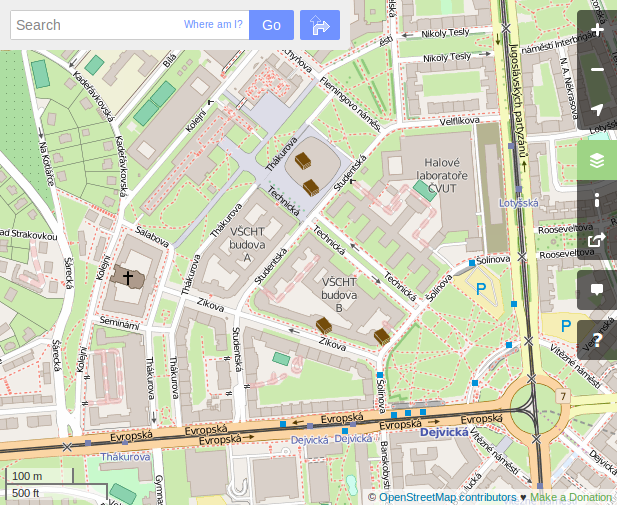
\includegraphics[width=11.5cm]{pictures/osm_standard.png} 
    \caption{Standardní mapa (Standard)}
    \label{fig:standard}
\end{figure}

\begin{figure}[H]
    \centering
    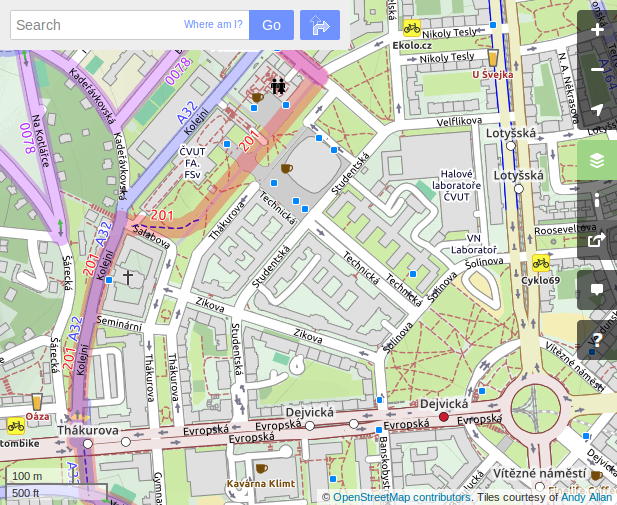
\includegraphics[width=11.5cm]{pictures/osm_cyclemap.png} 
    \caption{Cyklistická mapa (Cycle Map)}
    \label{fig:cycle}
\end{figure}

% new list

\begin{figure}[H]
    \centering
    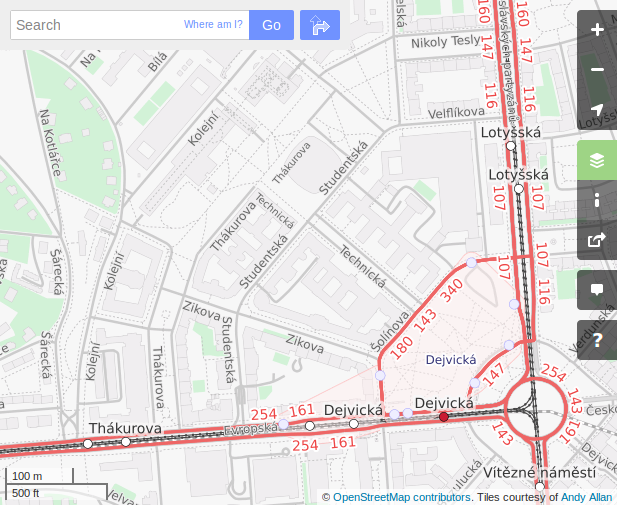
\includegraphics[width=11.5cm]{pictures/osm_transport.png} 
    \caption{Transport Map}
    \label{fig:transport}
\end{figure}

\begin{figure}[H]
    \centering
    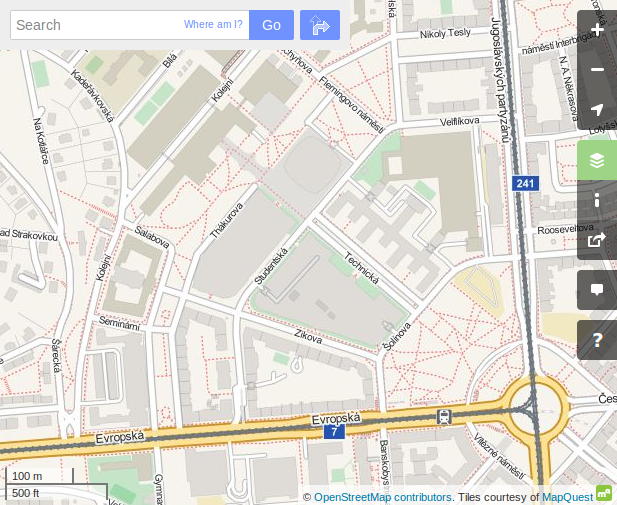
\includegraphics[width=11.5cm]{pictures/osm_mapquest.png} 
    \caption{MapQuest Open}
    \label{fig:mapquest}
\end{figure}

% new list

\begin{figure}[H]
    \centering
    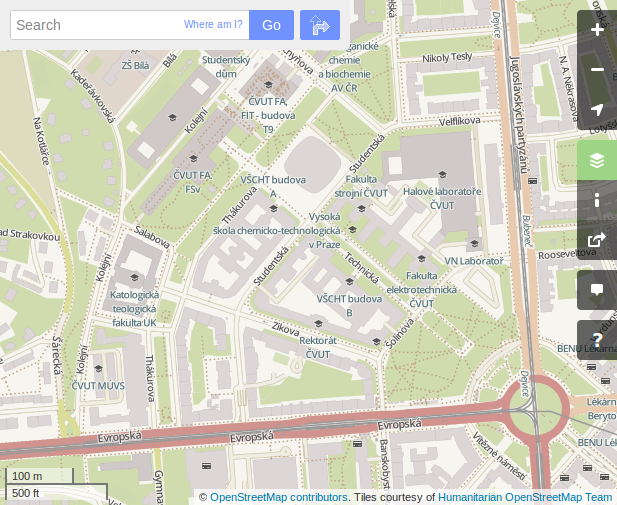
\includegraphics[width=11.5cm]{pictures/osm_humanitarian.png} 
    \caption{Humanitární mapa (Humanitarian)}
    \label{fig:humanitarian}
\end{figure}

\begin{figure}[H]
    \centering
    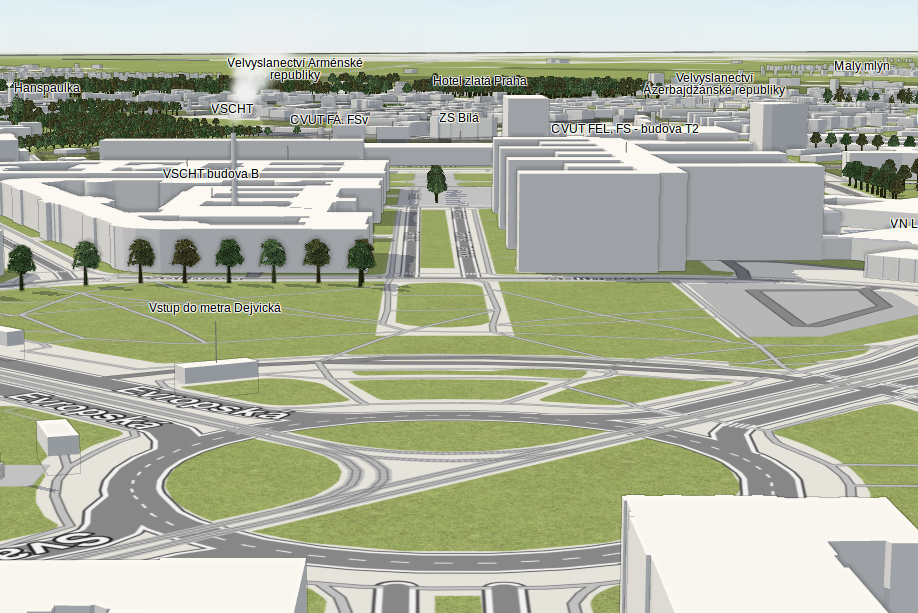
\includegraphics[width=11.5cm]{pictures/F4.png} 
    \caption{projekt F4 (zdroj \url{http://demo.f4map.com/}}
    \label{fig:F4}
\end{figure}

% new list

\chapter{Diagramy}
\label{digramy}

\begin{figure}[H]
  \centering
  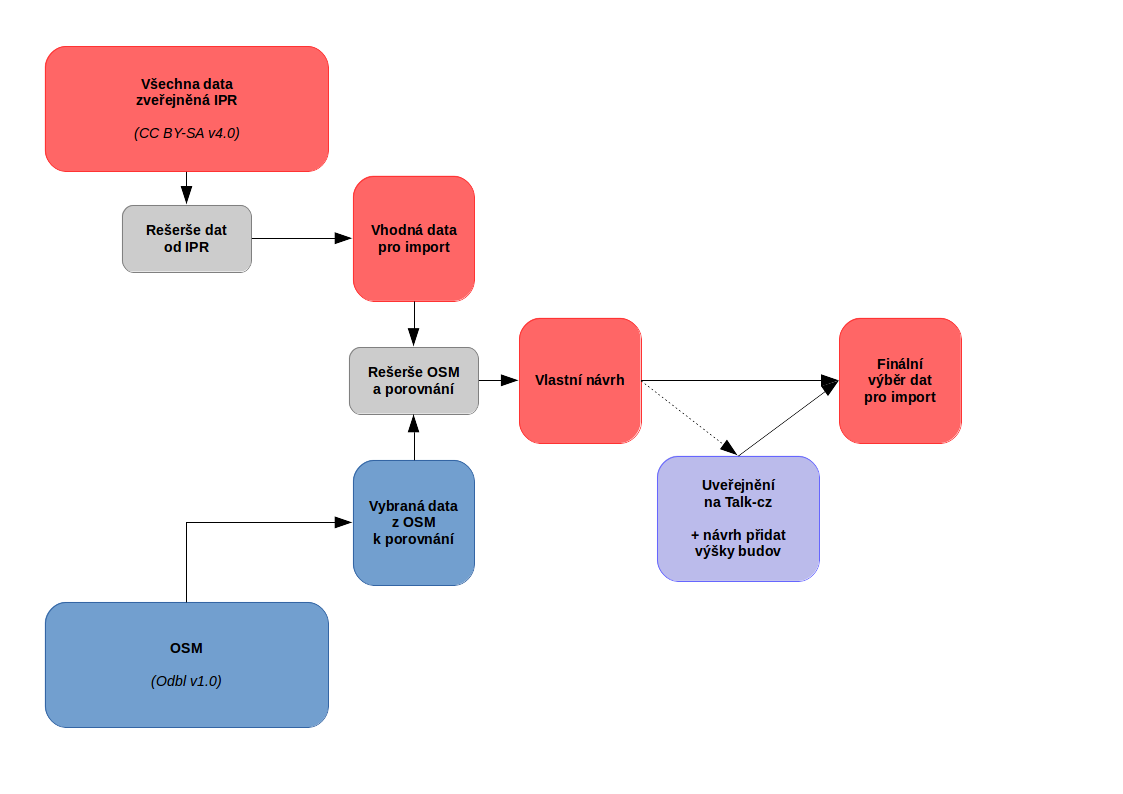
\includegraphics[scale=0.60,angle=90]{pictures/WorkFlow.png}
  \caption{Diagram postupu práce.}
  \label{fig:diagram_workflow}
\end{figure}

\begin{figure}[H]
  \centering
  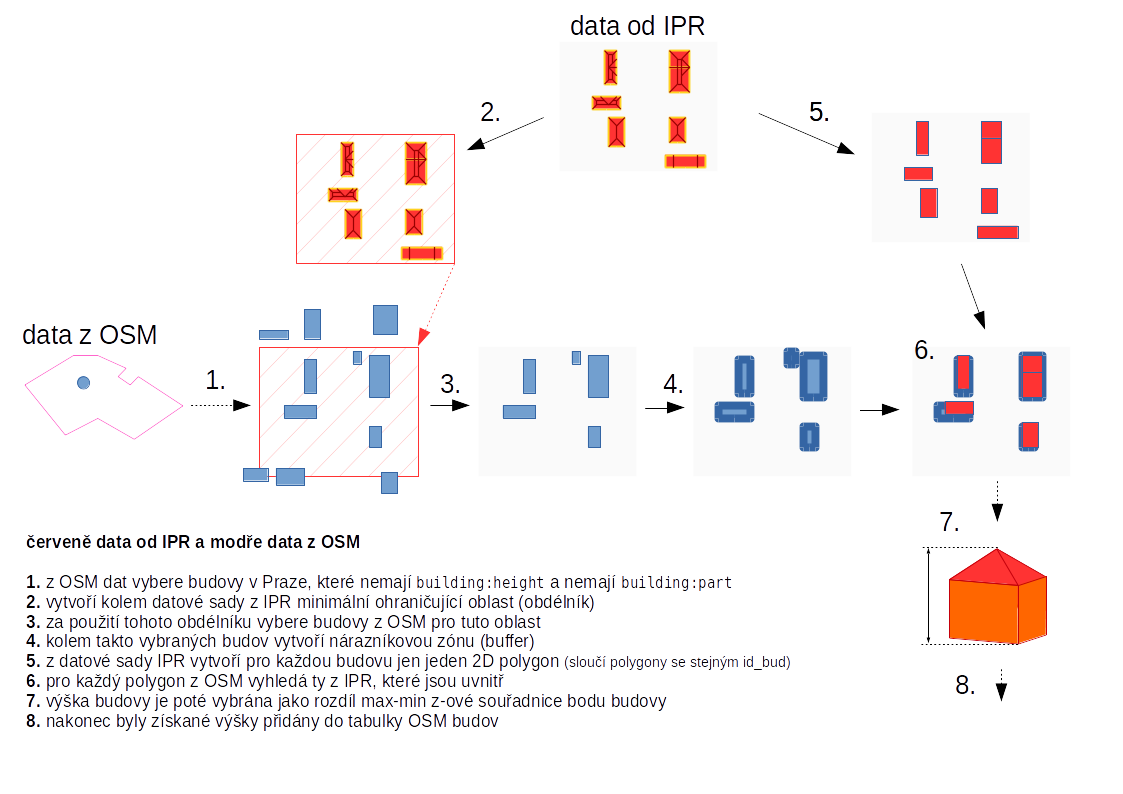
\includegraphics[scale=0.60,angle=90]{pictures/diagram_building_height.png}
  \caption{Diagram postupu práce pro získání výšky budov.}
  \label{fig:diagram_building}
\end{figure}

% new list

\chapter{Obsah CD}
\label{priloha-obsahCD}
\setlength{\unitlength}{.5mm}
\begin{picture}(250, 220)

  \put(  0, 212){\textbf{.}}

  \put(  1, 200){\line(0, 1){5}}
  \put(  1, 200){\line(1, 0){10} {\textbf{ src}}}  

      \put( 16, 190){\line(0, 1){8}}
      \put( 16, 190){\line(1, 0){10} {\textbf{ iprdownloader}}}
      \put(150, 190){ zdrojové soubory programu}

          \put( 29, 180){\line(0, 1){8}}
          \put( 29, 180){\line(1, 0){10} { IprBase.py}}
          \put( 29, 170){\line(0, 1){10}}
          \put( 29, 170){\line(1, 0){10} { IprPg.py}}
          \put( 29, 160){\line(0, 1){10}}
          \put( 29, 160){\line(1, 0){10} {\textbf{ Iprdownloader.py}}}

      \put( 16, 150){\line(0, 1){40}}
      \put( 16, 150){\line(1, 0){10} {\textbf{ pg}}}
      \put(150, 150){ zdrojové kódy shell skriptu}      

          \put( 29, 140){\line(0, 1){8}}
          \put( 29, 140){\line(1, 0){10} { pgis\_osm\_bp.style}}
          \put(150, 140){ vlastní schema dat z OSM}
          \put( 29, 130){\line(0, 1){10}}
          \put( 29, 130){\line(1, 0){10} { upgrade\_pgis\_osm\_bp.sql}}
          
      \put( 16, 120){\line(0, 1){30}}
      \put( 16, 120){\line(1, 0){10} {\textbf{ sql}}}
      \put(150, 120){ zdrojové kódy sql dump}
            
          \put( 29, 110){\line(0, 1){8}}
          \put( 29, 110){\line(1, 0){10} { buildins.sql}}
          \put( 29, 100){\line(0, 1){10}}
          \put( 29, 100){\line(1, 0){10} { park\_and\_ride.sql}}
          \put( 29,  90){\line(0, 1){10}}
          \put( 29,  90){\line(1, 0){10} { parkomat.sql}}
          \put( 29,  80){\line(0, 1){10}}
          \put( 29,  80){\line(1, 0){10} { recycling\_centre.sql}}
          \put( 29,  70){\line(0, 1){10}}
          \put( 29,  70){\line(1, 0){10} { toilets.sql}}          
          
  \put(  1,  60){\line(0, 1){140}}
  \put(  1,  60){\line(1, 0){10} {\textbf{ text}}}

      \put( 16,  50){\line(0, 1){8}}
      \put( 16,  50){\line(1, 0){10} {\textbf{ latex}}}
      \put(150,  50){ zdrojové soubory textu této práce}
      \put( 16,  40){\line(0, 1){10}}
      \put( 16,  40){\line(1, 0){10} { martin-jakl-bp-2016.xls}}
      \put(150,  40){ anotace práce}
      \put( 16,  30){\line(0, 1){10}}
      \put( 16,  30){\line(1, 0){10} { martin-jakl-bp-2016.pdf}}
      \put(150,  30){ tento text}
      \put( 16,  20){\line(0, 1){10}}
      \put( 16,  20){\line(1, 0){10} { zadani-oficialni.jpeg}}
      \put(150,  20){ naskenované oficiální zadání práce}
\end{picture}


% Konec dokumentu
\end{document}
